\documentclass{article}
\usepackage{graphicx}
\usepackage{booktabs}
\usepackage{url}
\usepackage{enumitem}
\usepackage{cite}
\usepackage{amsmath,amssymb,amsfonts}
\usepackage{algorithmic}
\usepackage{graphicx}
\graphicspath{{./images/}}
\usepackage{rotating}
\usepackage[hidelinks]{hyperref}
\usepackage{geometry}
\usepackage{textcomp}
\usepackage[dvipsnames]{xcolor}
\usepackage{booktabs}
\usepackage{caption}
\usepackage{xspace}
\usepackage{float}
\usepackage{marginnote}
\usepackage{tabularx}
\usepackage{changepage, threeparttable}
\usepackage{attrib}
\usepackage{svg}
\usepackage{multirow}
\usepackage[normalem]{ulem} % for strike through text \sout{asd}
\usepackage{listings}
\usepackage{listingsutf8}
\lstset{
    inputencoding=utf8,
basicstyle=\small\ttfamily,
columns=flexible,
breaklines=true,
keepspaces=false,
}
\geometry{margin=2.5cm}

\title{\textbf{Chirp-Vee2}}
\date{April 2026}
\author{}

\begin{document}
\begin{titlepage}
  \centering
  \vspace*{2cm}
  {\LARGE \textbf{Chirp-Vee2} \par}
  \vspace{0.5cm}
  {\large Course code: \textit{BSDSESM1KU} \par}
  \vspace{0.25cm}
  {\large May 2026 \par}
  \vspace{0.5cm}
  {\normalsize Exam Assignment by \par}
  \vspace{1.5cm}

  \begin{tabular}{ll}
    \toprule
    \textbf{Student} & \textbf{Email} \\
    \midrule
    Hassan Hamoud Al Wakiel   & \href{mailto:halw@itu.dk}{halw@itu.dk} \\
    Nicky Chengde Ye          & \href{mailto:niye@itu.dk}{niye@itu.dk} \\
    Madsemil Søndergaard Søgaard & \href{mailto:msso@itu.dk}{msso@itu.dk} \\
    David Kvistorf Larsen (Vee)     & \href{mailto:dakl@itu.dk}{dakl@itu.dk} \\
    \bottomrule
  \end{tabular}
\end{titlepage}

\tableofcontents
\section{System's Perspective}
\subsection{Design and architecture (Mads)}
\subsubsection{System deployment view}
\begin{figure}[H]
    \centering
    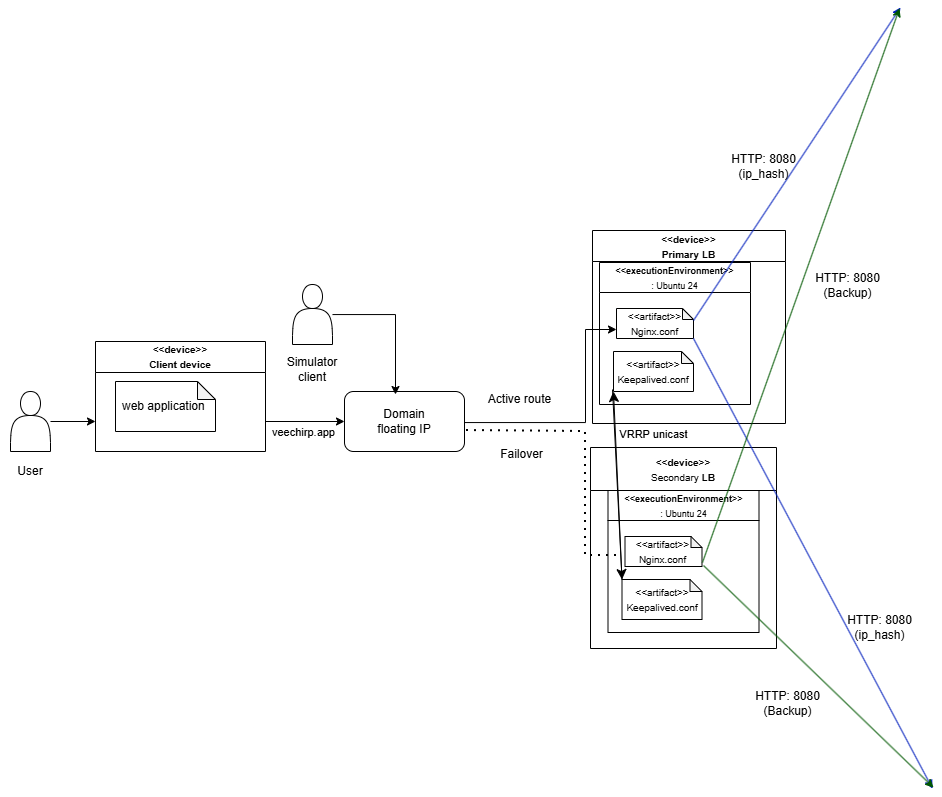
\includegraphics[width=1\linewidth]{images/1st_half_of_deployment.drawio.png}
    \caption{1st half of deployment diagram}
    \label{fig w1}
\end{figure}

The application is deployed across two independent Docker Swarm clusters on DigitalOcean, each consisting of one manager node and two worker nodes. Users access the system via veechirp.app, which resolves through DNS to a DigitalOcean floating IP address shared between two load balancer VMs running Nginx and Keepalived. Under normal operation the primary load balancer holds the floating IP. If it fails, Keepalived detects this via a VRRP unicast heartbeat over the private network and reassigns the IP to the secondary. Nginx distributes requests across both swarm managers using IP hash-based load balancing, which in turn forward traffic to the worker nodes running the application replicas.

\begin{figure}[H]
    \centering
    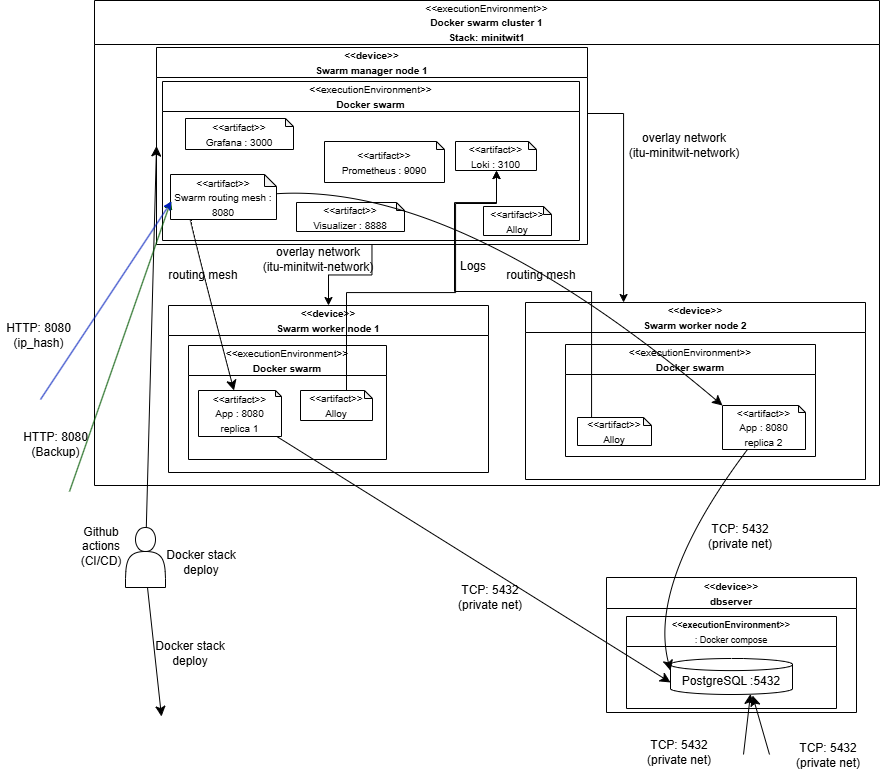
\includegraphics[width=1\linewidth]{images/DeploymentDiagramLight2ndHalf.drawio.png}
    \caption{2nd half of deployment diagram}
    \label{fig w1}
\end{figure}

On each manager node, Prometheus, Grafana, and Loki handle metrics and log aggregation, while Grafana Alloy runs on every node to ship logs to Loki. All application replicas connect to a single shared PostgreSQL database on a dedicated VM over the private network. Deployments are triggered by GitHub Actions, which runs docker stack deploy against each swarm manager. See full deployment diagram in the appendix. 

\subsubsection{HTTP Request Flow}

\begin{figure}[H]
    \centering
    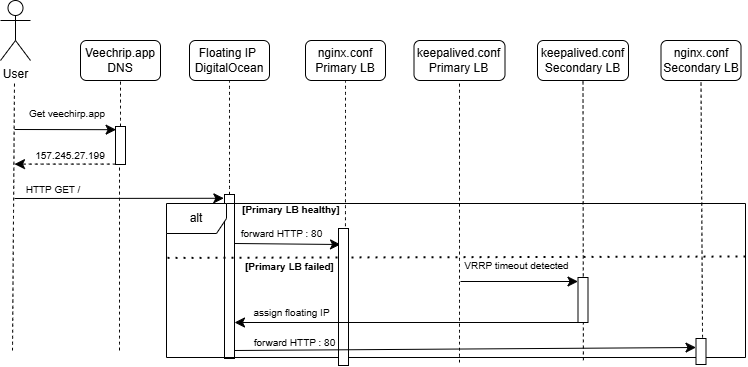
\includegraphics[width=1\linewidth]{images/Diagrams-1st half of seq.drawio.png}
    \caption{1st half of sequence diagram of HTTP request flow}
    \label{fig w1}
\end{figure}

The sequence diagram illustrates the lifecycle of an incoming HTTP request through the minitwit infrastructure. When a user navigates to veechirp.app, their browser resolves the domain to the DigitalOcean floating IP via DNS. The request is then forwarded to the primary load balancer, where Nginx distributes it to one of the two swarm managers using IP hash-based load balancing. If the primary load balancer becomes unavailable, Keepalived detects the failure through its VRRP heartbeat and reassigns the floating IP to the secondary load balancer, which takes over traffic.

\begin{figure}[H]
    \centering
    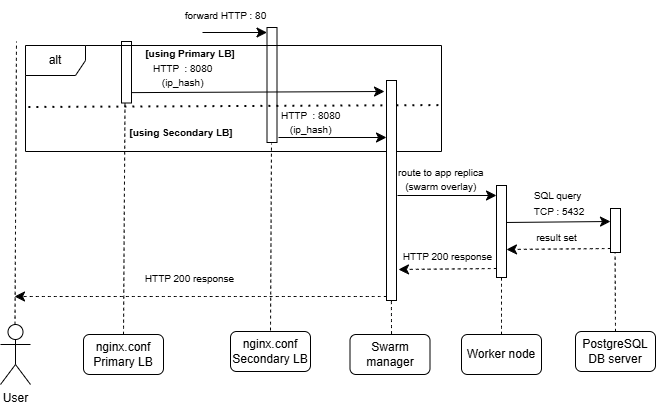
\includegraphics[width=1\linewidth]{images/Diagrams-2nd half of seq.drawio.png}
    \caption{2nd half of sequence diagram of HTTP request flow}
    \label{fig w1}
\end{figure}

Once the request reaches a swarm manager, it is forwarded through the swarm overlay network to a worker node running the application replica, which queries the PostgreSQL database and returns the response back up the chain to the user. Log entries generated during request handling are shipped asynchronously to Loki by Grafana Alloy running on the worker node. See full sequence diagram in the appendix. 
\\
\subsection{Tools and technologies (Hassan)}
The following is a list of technologies technologies and what they are used for:
\begin{enumerate}
    \item \textbf{.NET 10.0}: Used to write the Chirp application in C\#.
    \item \textbf{Docker}: Docker is used for running our application in deployment, horizontal scaling with Docker swarm, and blue-green deployment strategy.
    \item \textbf{Prometheus}: Used for collecting, storing and quering data for monitoring.
    \item \textbf{Loki}: Used for collecting, storing and quering data for logging.
    \item \textbf{Alloy}: Used to scrape logs from docker containers, and send them to Loki.
    \item \textbf{Grafana}: Used as an visualization tool for monitoring and logging.
    \item \textbf{Vagrant}: Creating and provisioning virtual machines.
    \item \textbf{SonarQube}: used as static analysis tool.
    \item \textbf{Codacy}: used as static analysis tool.
    \item \textbf{Hadolint}: used as linting for dockerfiles in CI/CD.
    \item \textbf{Shellcheck}: used as linting for shell scripts in CI/CD.
    \item \textbf{GitHub}: Used as version control, and for running CI/CD pipelines (workflows and actions).
    \item \textbf{Docker scout}: scans for docker image vunerabilities.
    \item \textbf{Python}: Used for utility files.
    \item \textbf{Ubuntu-22}: Used as operative system to host virtual machines.
    \item \textbf{Nginx}: Used for load balancers and reverse proxies.
    \item \textbf{Keepalived}: Used for high availability setup to create master and backup load balancer.
    \item \textbf{Shell scripts}: Used for to collect commands to provision virtual machines.
    \item \textbf{Digital ocean}: Used as cloud provider for VPS's, floating IP's.
    
\end{enumerate}
\subsection{Assessment of current state}
\subsubsection{SonarQube}
\textbf{Issues (Mads)} \\
 The large majority of issues reported by SonarQube are related to either the simulator or the Chirp project from our BDSA project. We decided not to focus on these issues and rather spend time on issues we are responsible for. The last remaining issues are related to SonarQube preferring '[[' over '[' because it is a shell keyword rather than a standard command, which eliminates common syntax errors and enables advanced features. We decided not to focus on fixing these issues and instead focus on implementing new features.
\\\\
\textbf{Security Hotspots (Hassan)}\\
SonarQube mentions in multiple of the dockerfiles that images might run as with root as default user. This is a security issue of medium priority. SonarQube suggest using the USER statement in our dockerfiles. Not doing this is a security risk, and goes against the principle of least privilege. it would've been a good thing to do in the future as it is a good practice and strengthens the security. Some lower priority security issues tells us to use full commit SHA for our dependencies for our github workflows for example:
"uses: docker/build-push-action@v6". This is another good practice if the author of the third-party action wasn't trustworthy, however the author is docker themselves. It's likely that any new commit is a bug fix.
\subsubsection{Codacy}
The most relevant things codacy complained about were also mentioned by SonarQube. Otherwise it was irrelevant things such as legacy code and BDSA.
\subsubsection{linters}
The other linters in our CI/CD, meaning hadolint and Shellcheck had no complaints.
\subsubsection{Domain (Nicky)}
An issue was discovered with access to the minitwit application through the veechirp.app domain because of issues with decrypting an antiforgery token. The full exception log is included in the appendix, but important parts are the `System.Security.Cryptography.CryptographicException´ and ´AntiforgeryValidationException´ lines. This might be related to CVEs discovered by Docker Scout shown below.
\begin{figure}[H]
    \centering
    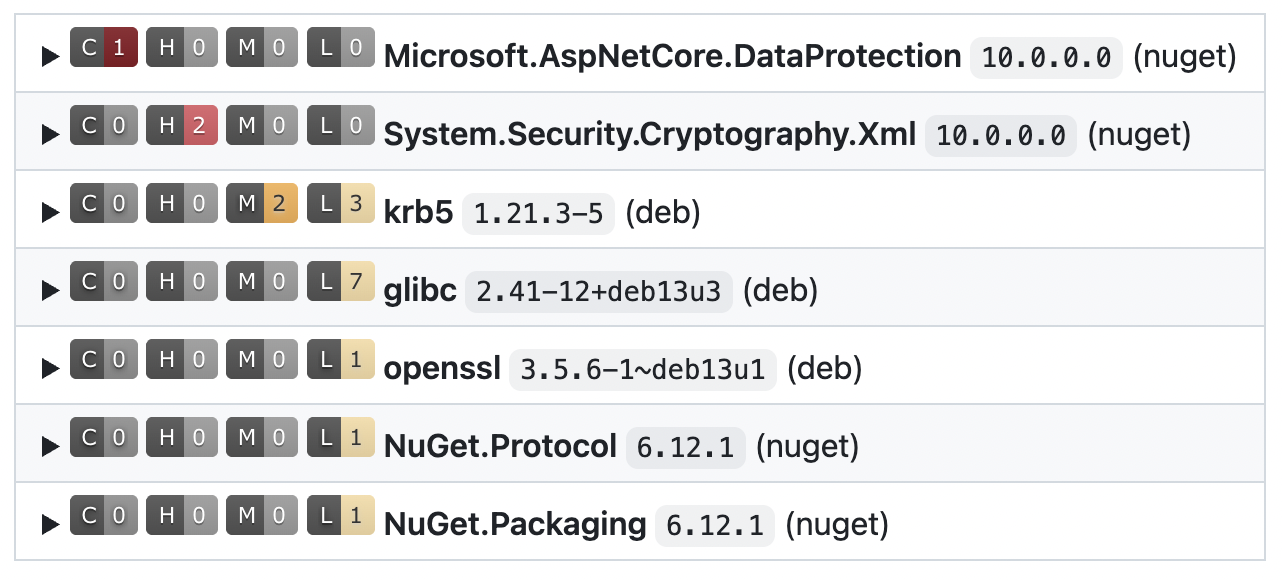
\includegraphics[width=1\linewidth]{images/DockerScoutCVE.png}
    \caption{CI/CD Docker Scout found CVEs}
    \label{fig:placeholder}
\end{figure}
\section{Process' perspective}
\subsection{CI/CD pipelines (Nicky)}
Two CI/CD pipelines that lint, do static code analysis and deploy the minitwit application exists.
\\\\
Linting and static code analysis runs when a pull request is opened and uses Hadolint, Shellcheck, Codacy and Sonarscanner to lint dockerfiles and shell scripts, and do static code analysis respectively. Hadolint and Shellcheck is defined in lint.yml, Sonarscanner is defined in sonarscanner.yml and Codacy is a GitHub app.
\begin{figure}[H]
    \centering
    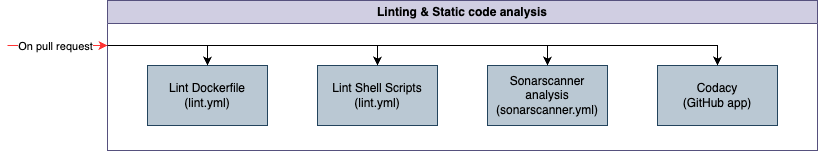
\includegraphics[width=0.75\linewidth]{images/lint-analysis.png}
    \caption{Linting \& Static code analysis}
    \label{fig:placeholder}
\end{figure}
The deployment pipeline is defined in deploy.yml. It tests Minitwit, builds and pushes Minitwit, Prometheus and Grafana to Docker Hub, runs Docker Scout analysis on Minitwit image, and deploys it all on the two Docker Swarm clusters (Not in this particular order). Releases are made manually every time something is pushed to main.
\begin{figure}[H]
    \centering
    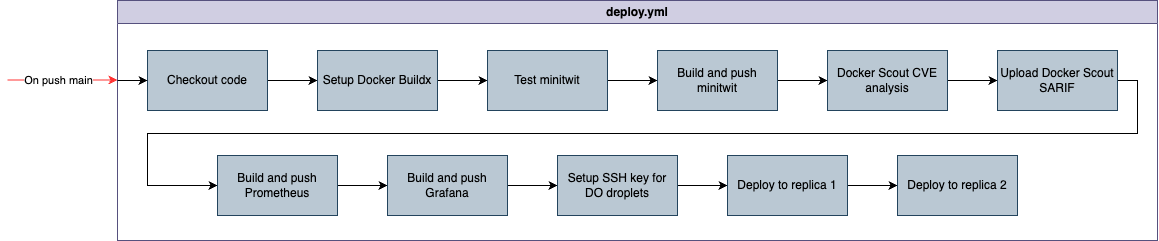
\includegraphics[width=1\linewidth]{images/deploy.png}
    \caption{Deployment pipeline}
    \label{fig:placeholder}
\end{figure}
\subsection{Monitoring \& Logging (Nicky)}
Monitoring is done utilizing Prometheus a metrics tool, and Grafana for visualizing and monitoring. How it works is that Prometheus pulls metrics from the minitwit containers through the `/monitoring/metrics` endpoint, and then Grafana queries Prometheus for the data to be visualized.
\\\\
What is monitored is:
\begin{enumerate}
    \item Request duration for every route called.
    \item Average request duration for slowest routes called.
    \item Request duration for every route called.
    \item Central CRUD endpoints to the miniwit application; getMessages, postMessage, registerAuthor, followAuthor...
    \item Front page average response time.
    \item CPU load over time.
    \item Average CPU load for the last hour.
    \item Average CPU load for the last day.
    \item Registered users.
    \item Average followers per user.
\end{enumerate}
\begin{figure}[H]
    \centering
    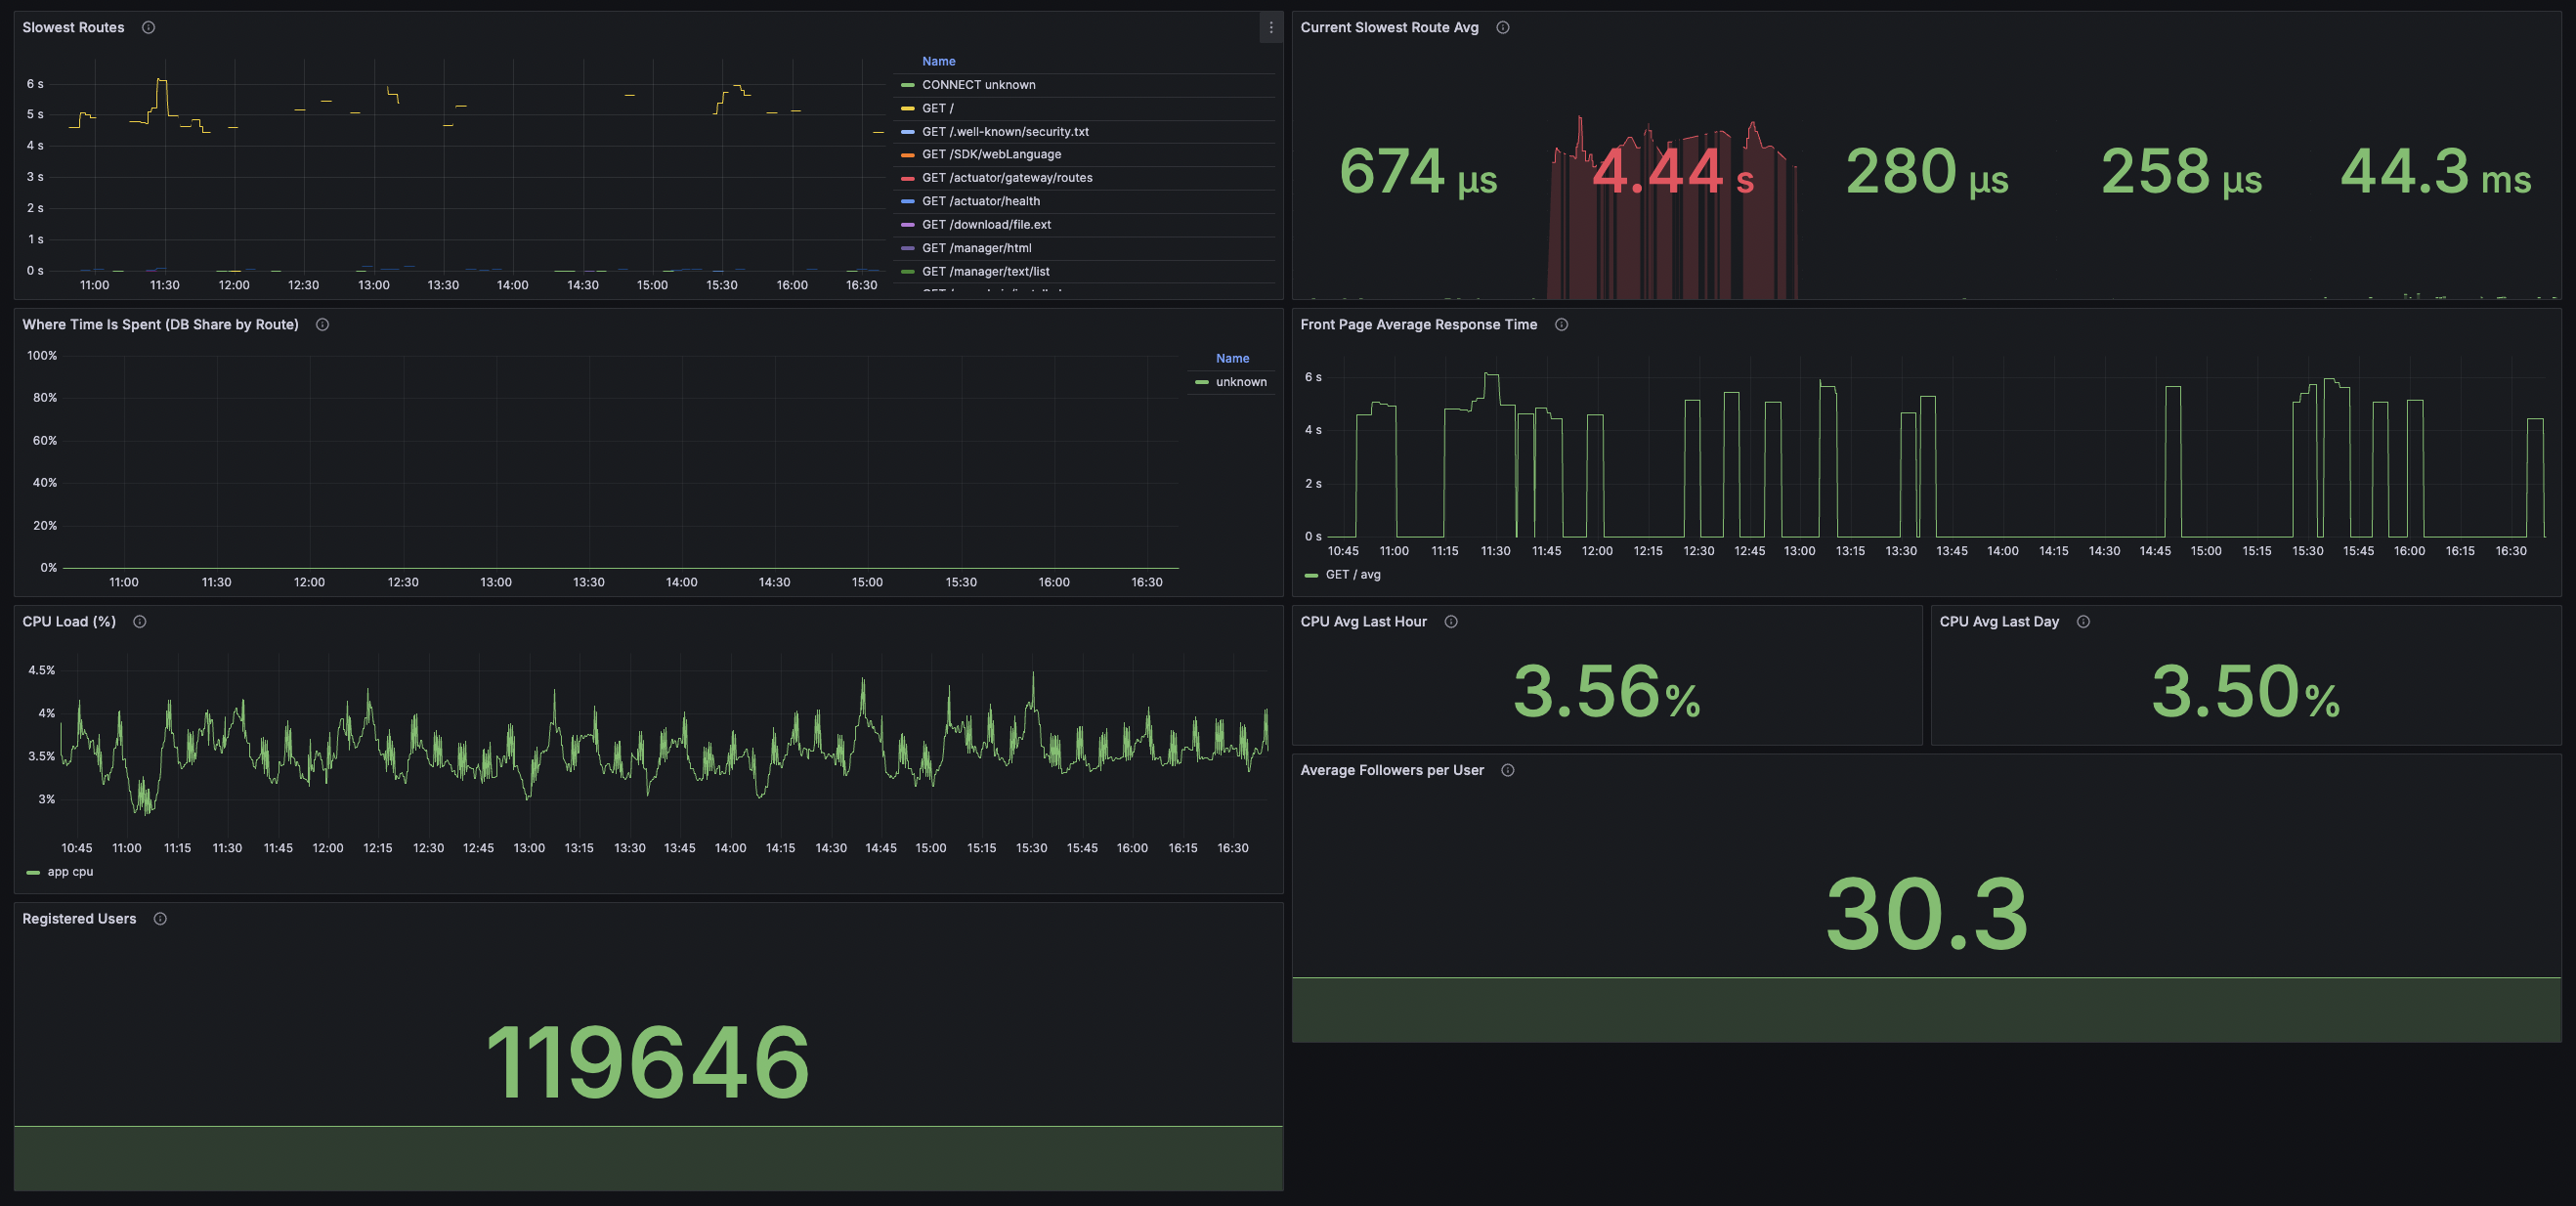
\includegraphics[width=1\linewidth]{images/Monitoring-dashboard.png}
    \caption{Monitoring}
    \label{fig w1}
\end{figure}
Logging is done by using Alloy which is present on each container and scrapes container logs which are then sent to Loki. From Loki, Grafana can then query Loki and display the logs.
\\\\
What is logged is rather minimal but is:
\begin{enumerate}
    \item Grafana logs.
    \item Alloy logs.
    \item Loki logs.
    \item Prometheus logs.
    \item Standard Minitwit .NET logs and errors.
    \item Logins and login attempts to Chirp and their origins.
\end{enumerate}
\begin{figure}[H]
    \centering
    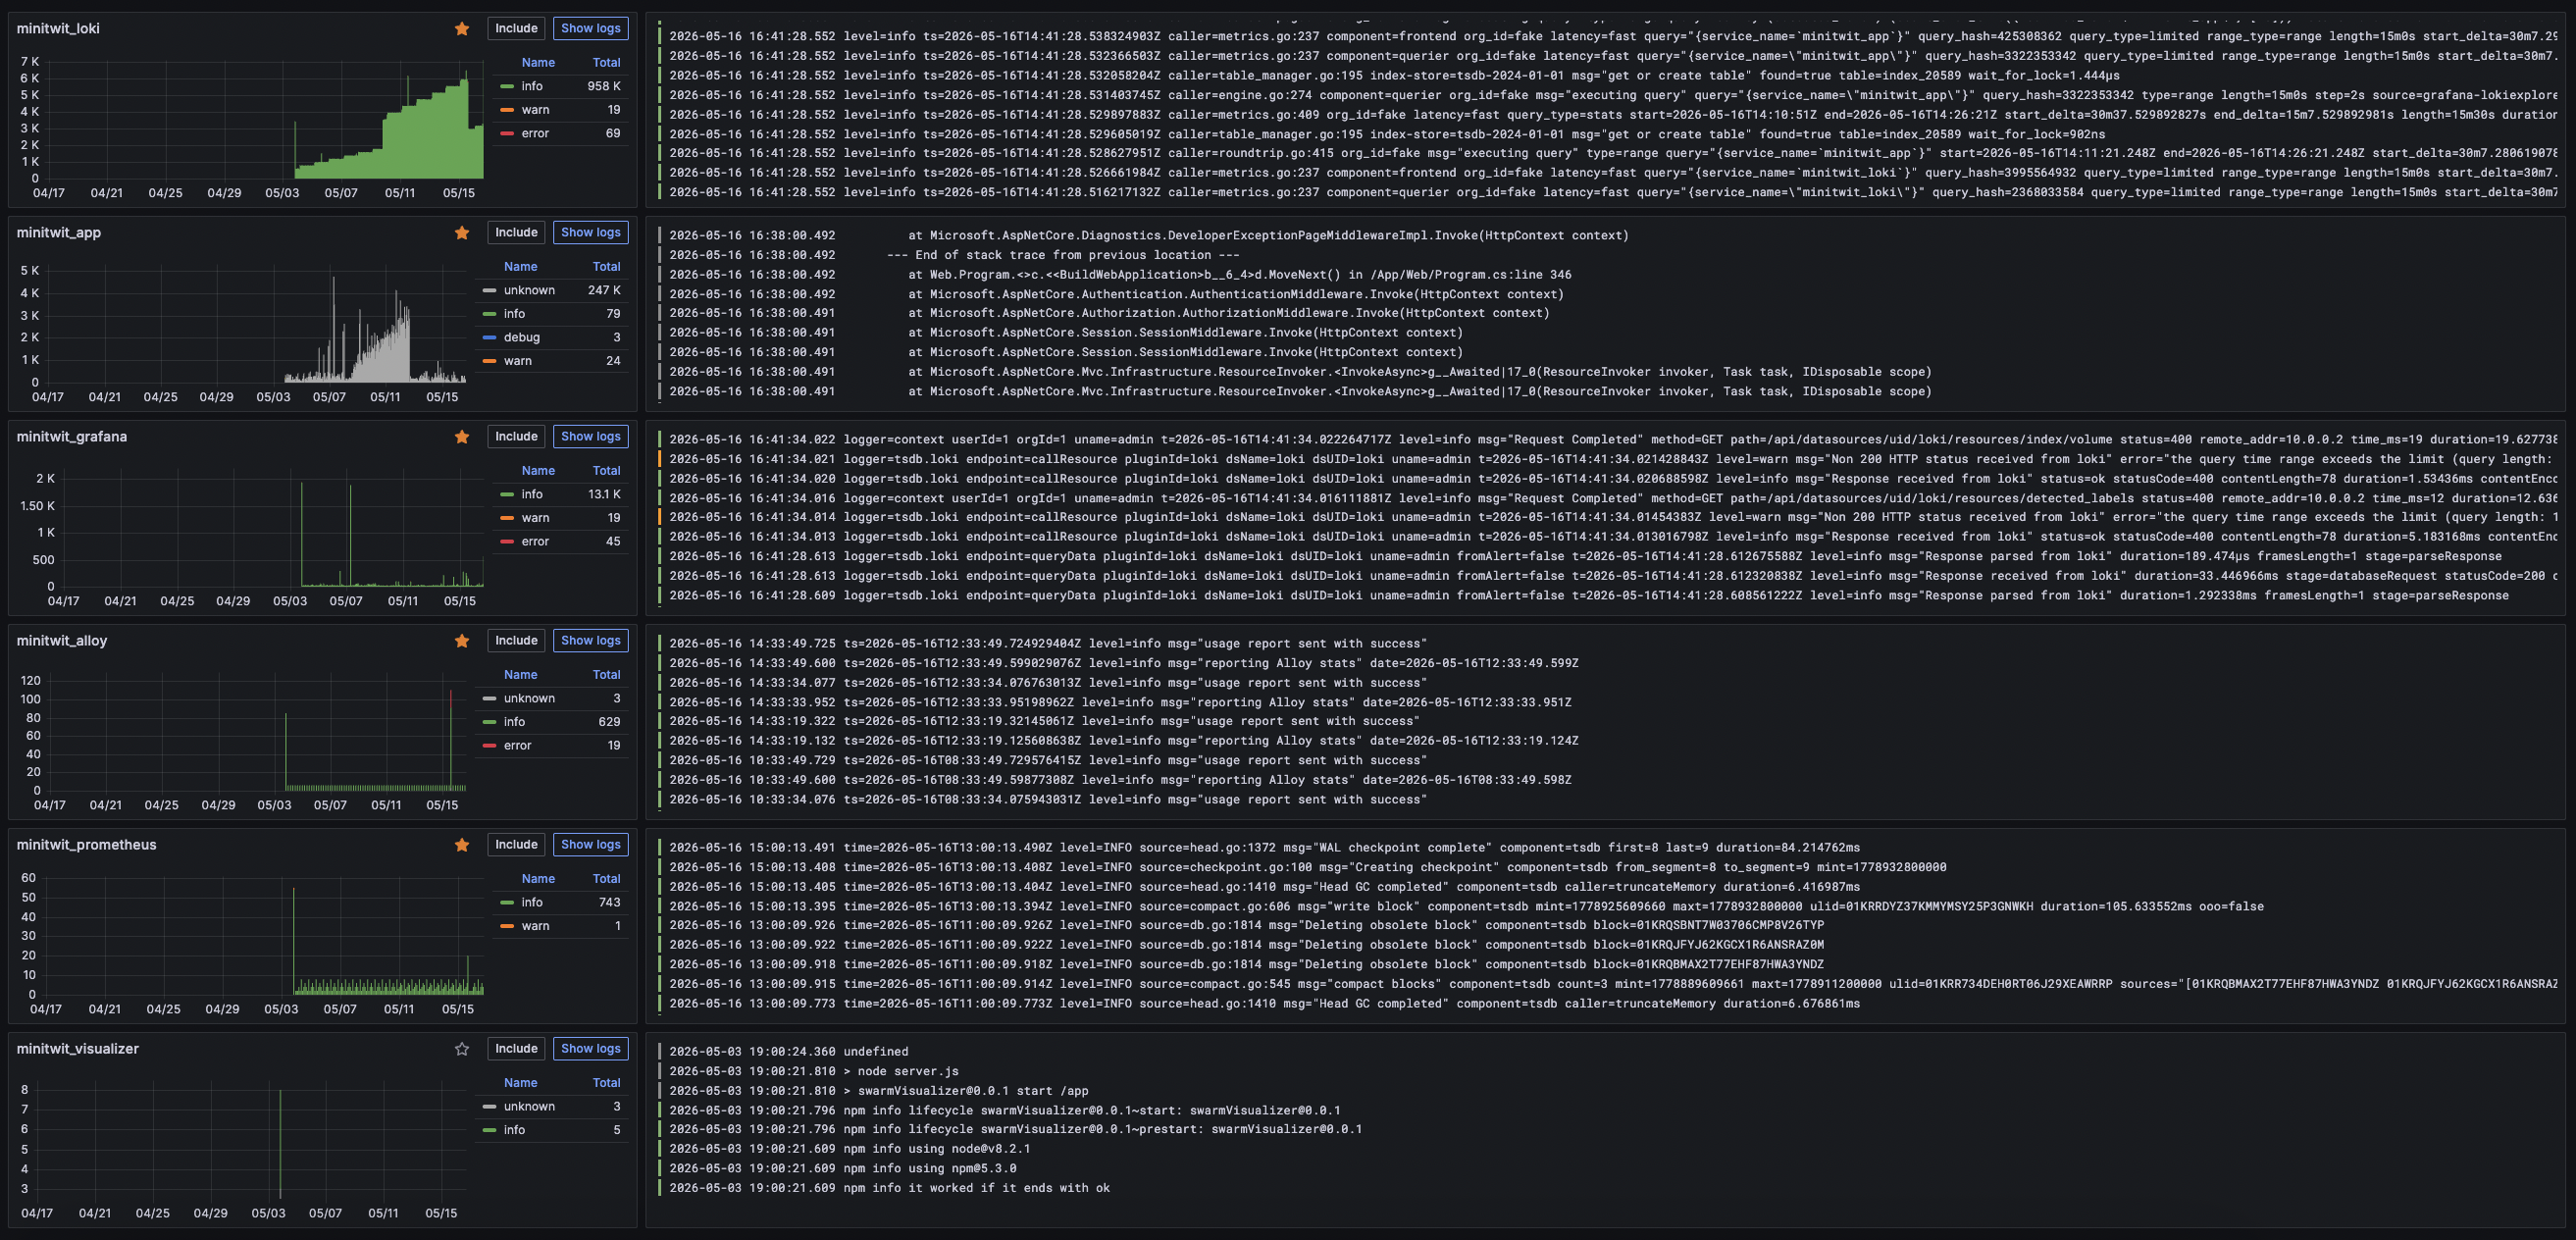
\includegraphics[width=1\linewidth]{images/Logging-dashboard.png}
    \caption{Logging}
    \label{fig w1}
\end{figure}
Things that could have been added to the logging was crossed resource threshold and durations. Another caveat is that no centralised solution combining both swarm clusters monitoring and logs was implemented meaning that each cluster had a Grafana dashboard.
\\\\
The monitoring and logging architecture is illustrated below but a more detailed version can be seen in the full deployment diagram in the appendix.
\begin{figure}[H]
    \centering
    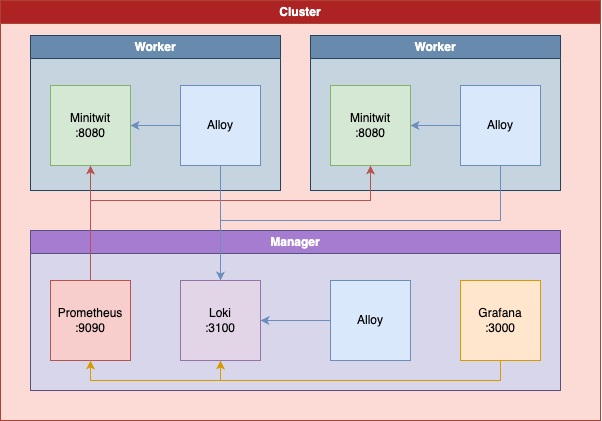
\includegraphics[width=0.75\linewidth]{images/Monitoring-Logging.png}
    \caption{Monitoring \& Logging}
    \label{fig w1}
\end{figure}
\subsection{Security (Hassan)}
For our application we have integrated a variety of security measures.
Our servers uses TLS. Using end-to-end encryption makes sure that information has not been tampered or with by a third party.
Along side performance enhancement reverse proxy also also strengthens the security of the service by hiding away the IPs for our servers. 
For our docker images uses hardened docker images along with docker scout scanning for vulnerabilities in the docker images in our CI/CD pipeline.
Our droplets also run a shell scripts, that we've written, that enables firewall on them. The scripts expose only the ports that are strictly necessary for the droplets to function.

\subsection{Availability and scaling (Vee + Hassan)}

\subsubsection{Load Balancers}
To ensure scaling and availability, we use two load balancers. These load balancers have a floating IP, which is set to our primary load balancer. When the primary load balancer crashes, the floating ip gets assigned to the backup load balancer. This makes sure that our website is still up and running even if the primary load balancer crash. \\
Our domain is naturally linked to the floating IP.

\begin{figure}[H]
    \centering
    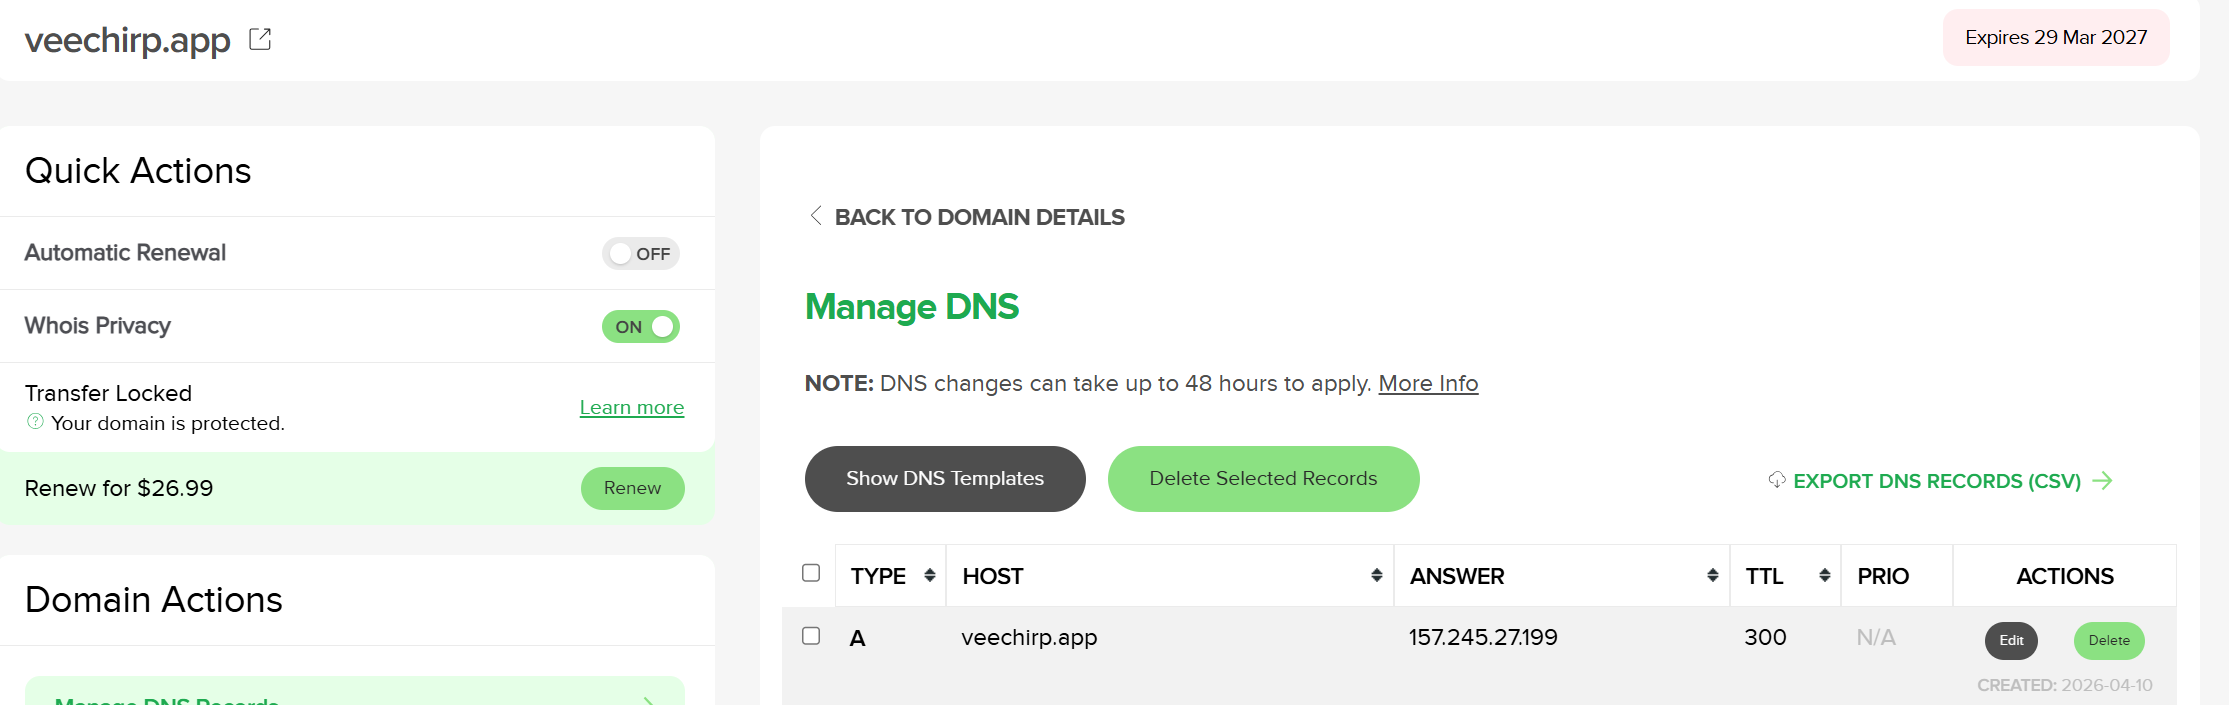
\includegraphics[width=1\linewidth]{images/domain.png}
    \caption{The Answer API for our domain}
    \label{fig w1}
\end{figure}

\subsubsection{Docker swarm}
How we scale is horizontally using docker swarm. In the vagrantfile before the load balancers are instantiated, two swarm managers droplets are created. Then two Swarm worker droplets are created for each of the two swarm managers, and attempt to join the swarm managers cluster. once they have joined, the manager distributes work among their workers and also act as a worker themselves. Figure \ref{docker swarm} is an illustration of how scaling and availability is implemented with domain, load balancers, and docker swarm (see appendix \ref{fig:fullDeployment} for more detail).

\begin{figure}[H]
    \centering
    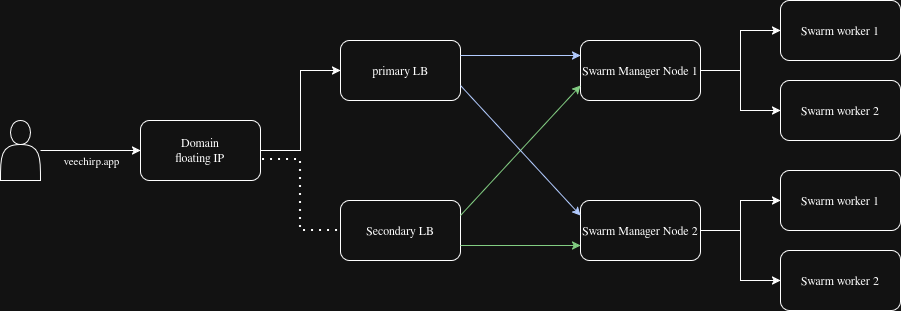
\includegraphics[width=1\linewidth]{images/ScalingAndAvailibity.png}
    \caption{Docker swarm}
    \label{docker swarm}
\end{figure}

\section{Reflection Perspective}
\subsection{Evolution and refactoring (Vee)}
To integrate the simulator, a simulator controller and new methods had to be added to comply with the provided API.
\\\\
When the application had to be scaled for availability, the Vagrantfile needed to be refactored to provision two load balancers and two minitwit applications.
\\\\
Observed in the logging system was collisions on cheepIds. Previously it was generated by checking the number of cheeps in the database and then incrementing. This was changed to auto generating by PostgreSQL. (Nicky)

\subsection{Operation and Maintenance (Vee)}
Maintenance wise, there were some cases. A big issue was the monitoring and logging system. Too much data was being logged, leading the server not being able to keep up. This was solved when Docker Swarm was introduced, thereby enabling distribution of workload. 
\\\\
Another issue was the domain setup. Initially, this was manually configured. But when two load balancers were introduced, there was an issue in obtaining a certificate for both. This was solved by copying the certificate from the master to the backup.

\section{Use of Generative AI (Vee)}
Generative AI was used to fix errors during the project. It was also used as a sparring partner for more difficult and hard to understand programs, especially when we are introduced to so many programs as we are in this course. 

\section{Absent team member}
We did not include Julián [juji] as a co author of the report since he did not help with writing it. Through the project work, Julián disappeared without communicating with the rest of the team until late in the project work (last week of lectures) and we have decided that we do not want to include him in the final exam project since he hasn't contributed to it.

\section{Appendix}

\subsection{Full sequence diagram}

\begin{figure}[H]
    \centering
    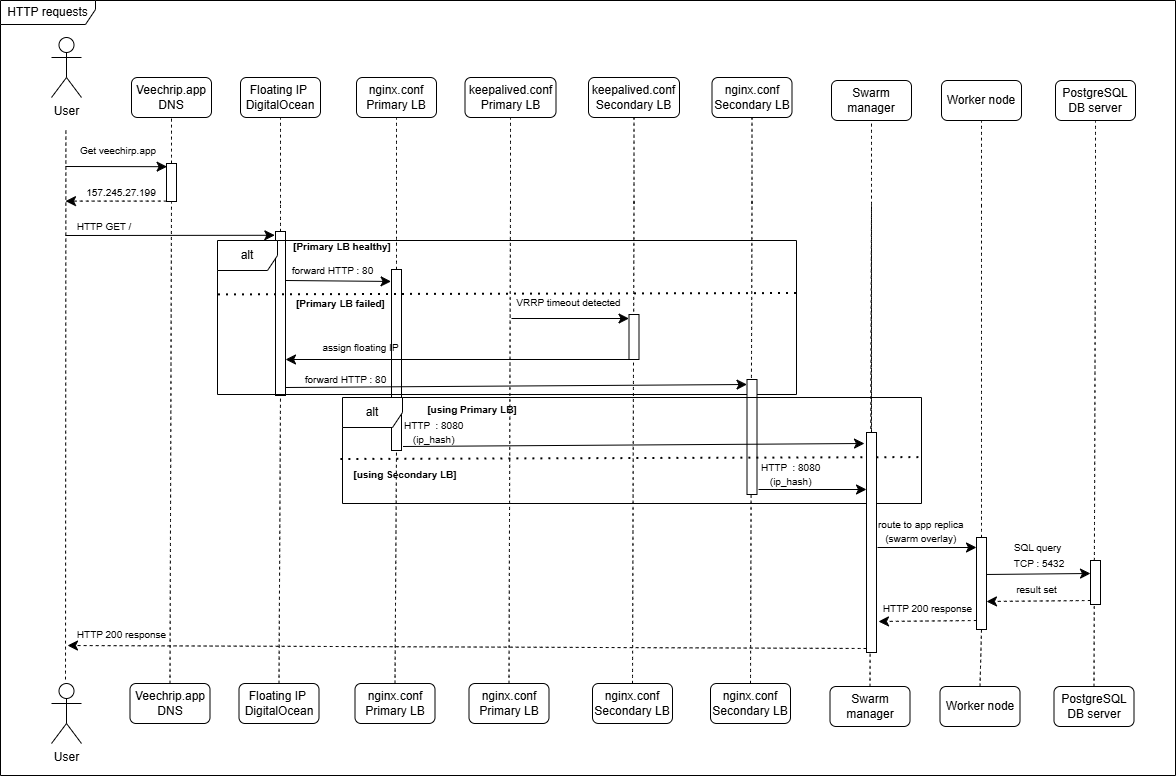
\includegraphics[width=1\linewidth]{images/SequenceDiagramLight.drawio.png}
    \caption{Sequence diagram of HTTP request flow}
    \label{fig:full sequence diagram}
\end{figure}


\subsection{Full deployment diagram}

\begin{sidewaysfigure}
    \centering
    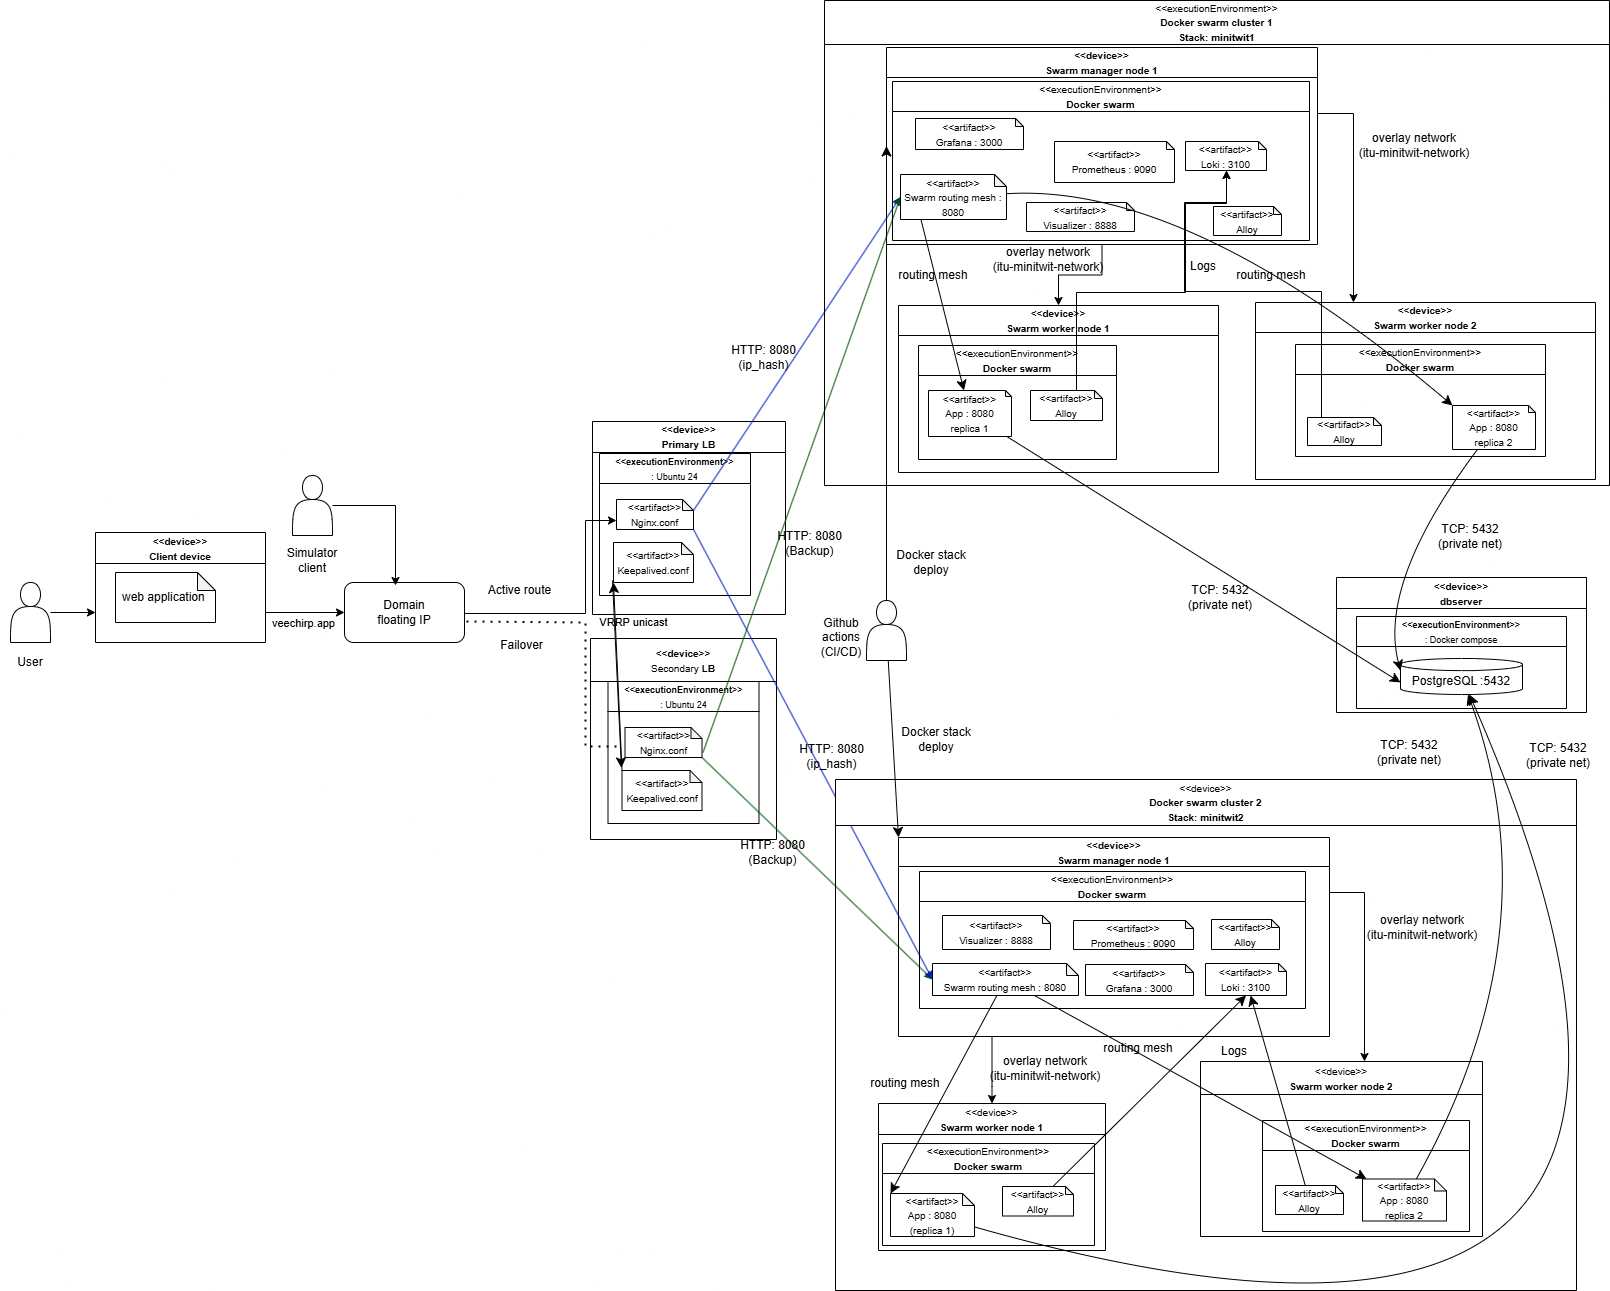
\includegraphics[width=\textheight, height=\textwidth, keepaspectratio]{images/DeploymentDiagramLight.drawio.png}
   \caption{DeploymentDiagram}
    \label{fig:fullDeployment}
\end{sidewaysfigure}
\newpage

\subsection{Antiforgery token exception (Nicky)}
\begin{lstlisting}[inputencoding=utf8]
	2026-05-17 19:20:12.394	
         at Microsoft.AspNetCore.Antiforgery.DefaultAntiforgeryTokenSerializer.Deserialize(String serializedToken)
	2026-05-17 19:20:12.394	
         at Microsoft.AspNetCore.DataProtection.KeyManagement.KeyRingBasedDataProtector.Unprotect(Byte[] protectedData)
	2026-05-17 19:20:12.394	
       ---> System.Security.Cryptography.CryptographicException: The key {1a2764b8-194f-41b5-aca0-35ea8cb01595} was not found in the key ring. For more information go to https://aka.ms/aspnet/dataprotectionwarning
	2026-05-17 19:20:12.394	
      Microsoft.AspNetCore.Antiforgery.AntiforgeryValidationException: The antiforgery token could not be decrypted.
	2026-05-17 19:20:12.394	
      An exception was thrown while deserializing the token.
	2026-05-17 19:20:12.393	
fail: Microsoft.AspNetCore.Antiforgery.DefaultAntiforgery[7]
\end{lstlisting}

\end{document}